% Chapter 1

\chapter{Introduction} % Main chapter title
\label{sec:intro}

\label{Chapter1} % For referencing the chapter elsewhere, use \ref{Chapter1} 

%----------------------------------------------------------------------------------------

% Define some commands to keep the formatting separated from the content 
\newcommand{\keyword}[1]{\textbf{#1}}
\newcommand{\tabhead}[1]{\textbf{#1}}
\newcommand{\code}[1]{\texttt{#1}}
\newcommand{\file}[1]{\texttt{\bfseries#1}}
\newcommand{\option}[1]{\texttt{\itshape#1}}

%----------------------------------------------------------------------------------------

\section{Concept}

The sound systems field has, since its inception, always been a very active market, where the success of an idea always meant the development of hundreds of products, generating very lucrative opportunities for the parties involved. Today, there are a multitude of companies that provide home theater systems for very different price ranges. In the last few years many of these entities have started including advanced Digital Signal Processing (DSP) software in their higher-end loudspeakers, like using the environment their products are into to their own advantage, this with the goal of improving the overall experience. It is foreseeable that this trend will only expand with the advancing of technology and the rising ubiquity of computing.
\\
The increasing desire for including these technologies is motivated by the fact that DSP can dramatically improve the enjoyment of users listening to sounds, by simulating virtual environments (for instance the digital surround systems used in cinemas), highlighting some characteristics of an audio system, by, for instance, compensating some undesired characteristics of the speakers, or by deploying sound steering and room correction techniques that provide a more "personalized" experience to the end user.
\\
It is exactly this last point that shows much promise for future development, and the starting point for this thesis work.
\\
Specifically, this kind of personalized experience can be developed using Acoustic Contrast Control (ACC) methods, a technique that aims to control the total amount of sound pressure in a limited zone of space. These regions, also called sound zones, are places where a user can be provided with personal audio, without the need for personal devices like headphones or earplugs.
\\
\\
The lowering of development and computational costs is starting to attract the industry into this field, which is becoming acquainted with the work made by the academia. This branch of research has in fact existed since the beginning of the $21^{th}$ century ~\parencite{choi_generation_2002},  but has seen a full blooming in the last $6-8$ years, with the development and improvement of advanced ACC techniques ~\parencite{elliott_robustness_2012,schellekens_time_2016,cai_time-domain_2014,chang_realization_2009}.
\\
\\
Proceeding into this reading it will appear clear how such a concept might prove useful in many, varied scenarios, ranging from entertainment to quality of life improvement. Imagine, for instance, a scenario of a discotheque, or some other environment where the music is very loud. There might be some areas, like the bar, or the smoking room, where the loud music sounds can be greatly reduced to let the customers socialize without having to struggle to understand each other. Or else, imagine hospital patients with head trauma that might want to entertain themselves with TV or music, but cannot use headphones. They might find great benefit from such system by being able to find comfort without disturbing other patients in neighboring beds. These are just two of the many application scenarios that can give the reader an idea how big and full of potential the market for acoustic contrast might be.
\\
\\
This thesis will demonstrate the feasibility of the development of an acoustic contrast method that, within the limits of its implementation, and with the expense of moderate computational time by a multi-core desktop PC, is able to generate, through the emission of finely tuned soundwaves, areas where the total acoustic energy is controlled. In this thesis project the scenario considered is the one with two zones, one acoustically "bright", where the desired sounds are reproduced and where the total acoustic energy is relatively high; And a "dark" zone, where the energy is kept as low as possible, resulting in an area of relative quiet. In order to control the sound pressure level inside these zones, a set of multiple loudspeakers is needed.
\\
The control is performed by determining a particular set of values that, when convolved with the output sound signal, will make the soundwaves interfere with each other inside the zone defined as dark, effectively creating silence. This is explained by the principle of superposition, which states that two waves that are incident generate a resulting wave that is equal to the vector sum of the two. If two ridges from two different waves at the same frequency meet at the same point, the amplitude of the resulting wave will be equal to the sum of the individual amplitudes, a phenomenon known as constructive interference. On the contrary if a ridge meets a valley, the resulting wave will be equal to the difference of the two, this effect is instead called destructive interference and is what we want to achieve in the dark zone.
\\
The objective is to obtain this interference, while keeping the sound level and frequency characteristics of the sounds in the bright zone as intact as possible, to do that we will calculate a set of weights to apply to the sounds coming out from a set of loudspeakers. The effectiveness of such a set of values, also called a filter, is tied to the specific room and the specific position of the sound zones. The term contrast is used to define the relative difference in decibels (dB) between the two zones. The configuration of said set can be arbitrary, but for this work, the speakers were mounted in a single line, at short distance one from the other, often referred to as an "array" of speakers. This was done with the objective of facilitating the transition from the test environment, to a more realistic one, by having a single instrument that is relatively easy to install or move.
\\
\\
The field of ACC is not free from challenges, and because of that, this thesis work tries to find the limits within the current state-of-the-art methods available in the academia and investigates one of the main problems in implementing such algorithms, namely the fact that having reflective surfaces in the room where acoustic contrast is performed, greatly increases the computational cost of finding a filter capable of providing a good result.
\\
Pretty much every surface inside a room is capable of reflecting sound, therefore solving this problem is paramount for the application of any ACC method in a real-world environment. In order to account for and therefore trying to eliminate the reflections generated by these surfaces, we need to find a longer set of weights. The increasing filter length is necessary so that the soundwaves that are reflected back into the sound zones, adding their energy, or modifying the frequency characteristics (also called frequency response) into our areas of interest, can be destroyed through interference. The length of the filter is directly proportional to the time of arrival of such reflections. This factor depends, of course, from the speed of sound and the distance that the waves have to travel. There are some variables that influence the speed of sound, such as the temperature of the surrounding environment (which is often the most important one), humidity and pressure; Since its value changes little for small changes of those conditions we will assume the speed of sound as a constant, having a value of $343$m/s.
\\
\\
Let's now make a simple example to explain how sound travels inside a room; Suppose that we have a 3x3x3 room with a small loudspeaker in it, positioned in a central position at the back of the room. Suppose now, that we have a microphone in the middle of said room. Now let's play a loud sound from the loudspeaker, for instance a single "bip" sound. If we start recording with the microphone at the same time the tone is being played, we will see the signal, corresponding to the arrival of the direct soundwave, being picked up by the microphone, after $~4.3$ms. This is because the instrument was set at a distance of $1.5$m and the sound has traveled at the finite speed of $~343$m/s.
\\
We'll also detect a second signal, after $~8.6$ms. Since the sound keeps traveling, it will in fact reach the wall on the other side of the room and part of it will be reflected back, passing by the microphone again, after having traveled a total distance of $3$m ($1.5$m after passing it and $1.5$m for coming back).
\\
In the meantime sound will also scatter in all directions and be reflected by the other walls, floor and ceiling. This will cause the presence of some amount of noise in the microphone measurement. The soundwaves will eventually die out, since they will disperse their energy while traveling through the air. Part of them will even be absorbed by the room surfaces, depending on the materials they are made of. The time of persistence of a sound, after it has been produced, is called reverberation time and is tied to the specific conditions of the room, like temperature, dimensions, building materials of the walls, etc.
\\
The figure below shows the overall concept at the base of this method.

\begin{figure}[H]
\centering
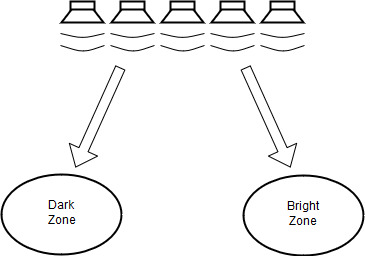
\includegraphics[width=10cm,height=10cm,keepaspectratio]{Figures/concept}
\decoRule
\caption[concept]{Overall concept. The idea is to use a set of loudspeakers to generate a difference in sound pressure level in two areas, the dark zone (low sound pressure) and the bright zone (high sound pressure). }
\label{fig:concept}
\end{figure}

In order to limit the disturbances created by said reflections, while developing an ACC method capable of acting on two soundzones, some experiments have been made, using an anechoic room as surrounding environment. This is a room specifically designed to dampen external sounds, as well as dramatically limiting the energy reflected back by the internal walls.
\\
There will necessarily be a divergence between the signal that has been inputted to the loudspeakers and the soundwave recorded by the microphones, this is due, mainly, to two different phenomena. The presence of reflections inside the room (that act as noise, as we said) and the nonlinear behavior of the loudspeakers. Any speaker, when solicited with a signal, will produce some unwanted sound components, that were not present in the original input.
\\
The impulse response (IR) is the figure that represents how the system (room, loudspeakers, other reflector surfaces) responds to said solicitations. It is derived by dividing the output of the system with its input. We will later see how the IR can be calculated for the specific system under test.
\\
\\
Going back to the ACC problem, this study analyses the feasibility of the approaches by the literature \parencite{cai_time-domain_2014,choi_generation_2002}, reproduces their results and proposes an evolution of the algorithm of choice that reduces the computational time required to find a filter(a set of weights) capable of generating some acoustic contrast. This is done in a specifically tailored scenario and with some limitations. The modified algorithm shows little degradation on the contrast figure with respect to the original solution proposed by \parencite{cai_time-domain_2014}. By measuring the impulse response and analyzing its characteristics it is possible to isolate the elements of the system that negatively affect the contrast (like reflective surfaces) and develop a filter that is able to limit their detrimental effect. This is achieved by splitting the impulse response (IR), the function that describes the characteristics of the room in question, in parts and creating an acoustic contrast filter for each one of these pieces, separately.
\\
\\
The scenarios used in the experiments will be progressively more difficult to control, since we will move from a simulated environment, to a real one, where it will be, at some point, added a reflective surface.
\\
The simulation will only consider two kinds of points, the ones that generate sound (which simulate some loudspeakers) and control points (which simulate some microphones), the physical implications of such objects will not be part of the experiment. Moving into the chamber, at the beginning, there will only be the necessary instruments to perform the experiments, namely the loudspeakers, used to reproduce the sound and the microphones, used to record the results of the experiments, together with the microphones power amplifiers. At a second time, a panel will also added inside the room, with the purpose of introducing a surface able to reflect sound. Before performing the ACC in the anechoic chamber some considerations about the speakers characteristics are made with a specifically designed experiment that analyses how different the sound signal, recorded by the microphones, is different with respect to the original one sent to them.
\\
In the end, the experiments will be repeated in a listening room, which is an environment much more similar to the living room of a common house, with tables, chairs, bookcases and other furniture. Needless to say, all of these objects will provide plenty of surfaces, that scatter sounds all over the room.
\\
\\
Summing up, the three scenarios where the ACC algorithm will be run are

\begin{enumerate}
  \item An anechoic chamber with the experiments hardware. 
  \item An anechoic chamber with the experiments hardware and a single reflective surface.
  \item A listening room with numerous surfaces that scatter sounds.
\end{enumerate}

The new technique devised in this work employs two ACC filters, developed using the same algorithm. These filters will tackle the problem of achieving contrast from two different sides, the first one will limit the acoustic energy in the dark zone coming \textbf{directly} from the loudspeakers.
\\
The second one will be applied in correspondence of the biggest source of reflections, which, in the case of point 2 of the above list, is also the only one having a clear and noticeable effect inside the room, while in point 3 the one taken into consideration and considered the "main" reflection will be one of the many present in the room.
\\
\\
The choice of having a maximum of two filters was not determined by some limitation in the algorithm, but rather dictated by a strive for consistency in the results, since there was a single surface in the anechoic chamber, a single reflection will be actively identified (and contrasted) in the listening room. Another problem, that will be discussed in chapter \ref{Chapter4} is that, while the reflection source is easily identifiable (and then separable) in the IR of the system in the anechoic chamber, it is not so easy to do so in the listening room. The windowing algorithm is discussed in section \ref{subsec:filtersplit}.
\\
Producing two different filters (one for the direct soundwave and one for the reflected one) takes much less computational time than calculating one single filter, which needs to be somewhat longer in order to be effective. Having a longer filter means that more samples of the IR are taken into account when calculating the ACC solution. The two shorter ones instead, can be merged and played back by the speakers, acting effectively in a similar manner as the longer one, but with a lower associated computational cost. This will necessarily introduce a decrease in the contrast figure, the magnitude of such trade-offs will be investigated in section \ref{subsec:filtersplit}.
\\
\\
The thesis objective can be overall synthesized as:
\\
\textbf{studying the ACC problem, focusing on the reflection problem, which is generated by having an object in the test environment that negatively impacts on the contrast achievable. This is done in a simplified scenario}.
\\
The solution proposed is then tested a listening room, where the validity of the concept is studied in a real-world scenario.
\\
\\
This work does not propose a definitive solution of the reflections problem, but takes a first step towards the resolution of the current limitations in the ACC algorithm chosen.
\\
The next few chapters will explain the specifics of the process, but at a glance, the work done can be summarized as follows,
\begin{itemize}
\item An algorithm able to perform ACC in wideband is selected. The algorithm was already available in literature \parencite{cai_time-domain_2014}. The proposed solution is reproduced.
\item The algorithm's performance is evaluated when changing some of its defining parameters (more details in \ref{sec:acc}).
\item The algorithm's limitations are analyzed. A variation that is capable to overcome at least some of its shortcomings is devised.
\item The modified version of the algorithm is tested, in some proposed use cases.
\end{itemize}

The following sections will describe the process carried out during the $4^{th}$ semester of the M.Sc. program at Aarhus University. The facilities used for this project were kindly made available by the Department of Engineering.

\section{Thesis structure}

In chapter \ref{Chapter2} the required theoretical background is presented to the reader. In section \ref{subsec:greenfct} is explained the propagation model that is the most popular for representing soundwaves moving in a spherical field. Later it is explained how a sound is generated by a loudspeaker and why its behaviour diverges from the ideal, linear case, by showing nonlinear distortions. In the end it is explained what ACC methods are and how do they work.
\\
\\
The experimental setup is described in details in chapter \ref{Chapter3}. In the chapter there are four sections that will explain the software, the hardware, the simulated and real environments used for the demonstrations. A detailed schema of the signal chain is presented in section \ref{subsec:sigchain}, that is how the digital, computer generated signal, arrives is reproduced and then recorded again by the microphones to be then converted back in a digital format. The power amplifiers, loudspeakers, microphones models and room dimensions are also listed in section \ref{sec:hw}.
\\
\\
Chapter \ref{Chapter4} analyzes the experiments in great detail, discusses and compares the results. Those are presented in progression as they have been performed, during the developing phase of this thesis work, in particular, the chapter is divided in experiments performed in the anechoic chamber (section \ref{sec:baccrd}) and the one made in the listening room (section \ref{sec:baccrdlisteningroom}). While progressing though them, the choices and trade-offs of the algorithm are investigated.
\\
\\
Finally, in chapter \ref{Chapter5} redacts the conclusions. It is there expressed what can be summarized from this work and where the main limitations lay. Moreover, a list of future improvements is proposed. 
